% =====================================================================
%  BÁO CÁO BÀI TẬP LỚN – TRỰC QUAN VÀ PHÂN TÍCH DỮ LIỆU
%  Đề tài 1: Superstore Sales Dataset – trình bày theo mẫu báo cáo BTL
%  Biên dịch bằng XeLaTeX (Overleaf: Menu -> Compiler -> XeLaTeX), chạy 2 lần.
% =====================================================================
\documentclass[12pt,a4paper]{article}

% Báo cáo cần XeLaTeX (hoặc LuaLaTeX). Trên Overleaf: Menu -> Compiler -> XeLaTeX -> Recompile.
\usepackage{iftex}
\ifPDFTeX
  \errmessage{BAO CAO CAN XELATEX: tren Overleaf chon Menu -> Compiler -> XeLaTeX roi bam Recompile}
  \stop
\fi

% ===================== THÔNG TIN CẦN ĐIỀN ============================
\newcommand{\HocPhan}{TRỰC QUAN VÀ PHÂN TÍCH DỮ LIỆU}
\newcommand{\DeTai}{XÂY DỰNG DASHBOARD PHÂN TÍCH DOANH SỐ BÁN LẺ SUPERSTORE}
\newcommand{\GiangVien}{Trần Hải Anh}
\newcommand{\Nhom}{Nhóm 12}
\newcommand{\Lop}{KHMT 18-01}
\newcommand{\NoiNam}{Hà Nội, năm 2026}
% =====================================================================

% ---------- Font: Times New Roman nếu máy có, nếu không dùng TeX Gyre Termes ----------
\usepackage{fontspec}
% Font nạp theo tên file (có sẵn trong TeX Live/Overleaf): nhanh và không phụ thuộc máy
\setmainfont{texgyretermes}[Extension=.otf, UprightFont=*-regular, BoldFont=*-bold,
  ItalicFont=*-italic, BoldItalicFont=*-bolditalic]
\setmonofont{lmmono10-regular.otf}[Scale=0.9]

% ---------- Lề theo mẫu: trên 2cm, dưới 2cm, trái 3cm, phải 1,5cm ----------
\usepackage[top=2cm,bottom=2.2cm,left=3cm,right=1.5cm,footskip=1cm]{geometry}
\usepackage{setspace}\setstretch{1.4}
\setlength{\parskip}{4pt}
\setlength{\parindent}{1cm}
\usepackage{indentfirst}

\usepackage{graphicx,float,booktabs,tabularx,array,multirow,longtable,amssymb}
\usepackage[table]{xcolor}
\usepackage{caption}\captionsetup{font=small,labelfont=bf,labelsep=period}
\usepackage{enumitem}\setlist{nosep,leftmargin=1.5em}
\usepackage{titlesec}
\usepackage{fancyhdr}
\usepackage{fancyvrb}
\usepackage{eso-pic}
\usepackage{tocloft}
\usepackage{tcolorbox}
\usepackage[hidelinks]{hyperref}

\definecolor{nau}{HTML}{823B0B}      % màu đường kẻ chân trang của mẫu
\definecolor{xam}{HTML}{555555}
\definecolor{nennhat}{HTML}{F2F2F2}

% ---------- Thuật ngữ tiếng Việt ----------
\renewcommand{\figurename}{Hình}
\renewcommand{\tablename}{Bảng}
\renewcommand{\contentsname}{MỤC LỤC}
\renewcommand{\listfigurename}{DANH MỤC HÌNH ẢNH}
\renewcommand{\listtablename}{DANH MỤC BẢNG BIỂU}
\renewcommand{\refname}{DANH MỤC TÀI LIỆU THAM KHẢO}

% ---------- Đánh số hình/bảng theo mục ----------
\counterwithin{figure}{section}
\counterwithin{table}{section}

% ---------- Tiêu đề mục kiểu mẫu: "1. Xác định bài toán" ----------
\titleformat{\section}{\fontsize{13}{18}\selectfont\bfseries}{\thesection.}{0.5em}{}
\titlespacing*{\section}{0pt}{14pt}{6pt}
\titleformat{name=\section,numberless}{\centering\fontsize{14}{18}\selectfont\bfseries}{}{0pt}{}
\titleformat{\subsection}{\normalsize\bfseries}{\thesubsection.}{0.5em}{}
\titlespacing*{\subsection}{0pt}{10pt}{4pt}
\titleformat{\subsubsection}{\normalsize\bfseries\itshape}{\thesubsubsection.}{0.5em}{}
\titlespacing*{\subsubsection}{0pt}{8pt}{2pt}

% ---------- Tiêu đề lớn căn giữa, in hoa (LỜI NÓI ĐẦU, MỤC LỤC, KẾT LUẬN...) ----------
\newcommand{\TieuDeLon}[1]{\clearpage\phantomsection\addcontentsline{toc}{section}{#1}%
  \begin{center}{\fontsize{14}{18}\selectfont\bfseries #1}\end{center}\vspace{4pt}}
\renewcommand{\cfttoctitlefont}{\hfill\fontsize{14}{18}\selectfont\bfseries}
\renewcommand{\cftaftertoctitle}{\hfill}
\renewcommand{\cftloftitlefont}{\hfill\fontsize{14}{18}\selectfont\bfseries}
\renewcommand{\cftafterloftitle}{\hfill}
\renewcommand{\cftlottitlefont}{\hfill\fontsize{14}{18}\selectfont\bfseries}
\renewcommand{\cftafterlottitle}{\hfill}
\renewcommand{\cftfigpresnum}{Hình~}\renewcommand{\cftfigaftersnum}{.}\setlength{\cftfignumwidth}{4.6em}
\renewcommand{\cfttabpresnum}{Bảng~}\renewcommand{\cfttabaftersnum}{.}\setlength{\cfttabnumwidth}{4.6em}
\renewcommand{\cftsecaftersnum}{.}
\renewcommand{\cftsubsecaftersnum}{.}
\renewcommand{\cftsecleader}{\cftdotfill{\cftdotsep}}
\setlength{\cftbeforesecskip}{3pt}

% ---------- Chân trang theo mẫu: đường kẻ đôi màu nâu + "Nhóm – Lớp" + số trang ----------
\pagestyle{fancy}\fancyhf{}
\renewcommand{\headrulewidth}{0pt}
\fancyfoot[L]{\small\textit{\Nhom\ – Lớp \Lop}}
\fancyfoot[R]{\small Trang \thepage}
\renewcommand{\footrule}{\vspace{-6pt}{\color{nau}\hrule height 0.5pt\vspace{1.5pt}\hrule height 1.6pt}\vspace{3pt}}
\fancypagestyle{plain}{\fancyhf{}\renewcommand{\headrulewidth}{0pt}%
  \fancyfoot[L]{\small\textit{\Nhom\ – Lớp \Lop}}\fancyfoot[R]{\small Trang \thepage}}

% ---------- Khung viền trang bìa ----------
\newcommand{\KhungBia}{\AddToShipoutPictureBG*{\AtPageLowerLeft{%
  \put(\LenToUnit{2.7cm},\LenToUnit{1.7cm}){{\setlength{\fboxrule}{3.5pt}\setlength{\fboxsep}{0pt}%
  \fbox{\rule{0pt}{26.4cm}\rule{17.1cm}{0pt}}}}}}}

% ---------- Hộp code, hộp nhận xét, ảnh chụp ----------
\fvset{fontsize=\small,frame=single,framesep=3mm,rulecolor=\color{black!25},xleftmargin=2pt,xrightmargin=2pt}
\newtcolorbox{nhanxet}{colback=nennhat,colframe=black!60,boxrule=0pt,leftrule=2.5pt,
  arc=0pt,left=6pt,right=6pt,top=4pt,bottom=4pt,fontupper=\small,
  before upper={\textbf{Nhận xét.}~}}
\setlength{\fboxsep}{0pt}\setlength{\fboxrule}{0.4pt}
\newcommand{\anh}[2][\linewidth]{%
  \IfFileExists{hinh/#2}{\fbox{\includegraphics[width=#1]{#2}}}%
  {\fbox{\parbox[c][4cm][c]{#1}{\centering\color{xam}Chèn ảnh chụp màn hình:\\ \texttt{hinh/\detokenize{#2}}}}}}
\graphicspath{{hinh/}}
\newcolumntype{Y}{>{\raggedright\arraybackslash}X}
\newcolumntype{C}{>{\centering\arraybackslash}X}
\newcommand{\usd}[1]{\$#1}

% =====================================================================
\begin{document}

% ============================ BÌA 1 ===============================
\begin{titlepage}
\KhungBia
\centering\setstretch{1.2}
{\fontsize{14}{17}\selectfont\bfseries BỘ GIÁO DỤC VÀ ĐÀO TẠO\\
\underline{TRƯỜNG ĐẠI HỌC ĐẠI NAM}\par}
\vspace{0.6cm}

\includegraphics[width=4.2cm]{logo.png}\par
\vspace{0.8cm}
{\fontsize{24}{28}\selectfont\bfseries BÀI TẬP LỚN\par}
\vspace{0.7cm}
{\fontsize{13}{18}\selectfont\bfseries TÊN HỌC PHẦN: \HocPhan\par}
\vspace{0.4cm}
{\fontsize{13}{19}\selectfont\bfseries ĐỀ TÀI: \DeTai\par}
\vspace{1.8cm}
\begin{flushleft}\hspace{1.6cm}\begin{minipage}{0.8\linewidth}\fontsize{13}{20}\selectfont
\textbf{Giáo viên hướng dẫn:}\ \ \GiangVien\\[4pt]
\textbf{Sinh viên thực hiện:}
\end{minipage}\end{flushleft}
\vspace{2pt}
{\fontsize{13}{17}\selectfont
\renewcommand{\arraystretch}{1.25}
\begin{tabular}{|>{\centering\arraybackslash}p{1cm}|>{\centering\arraybackslash}p{3.2cm}|>{\centering\arraybackslash}p{5cm}|>{\centering\arraybackslash}p{2.8cm}|}
\hline
\textbf{STT} & \textbf{Mã sinh viên} & \textbf{Họ và tên} & \textbf{Lớp} \\ \hline
1 & 1871040028 & Ngô Ngọc Sang & \Lop \\ \hline
2 & 1871040006 & Lê Thanh Đại & \Lop \\ \hline
3 & 1871040004 & Đỗ Quang Chính & \Lop \\ \hline
4 & 1871040013 & Võ Ngọc Hải & \Lop \\ \hline
\end{tabular}\par}
\vfill
{\fontsize{13}{17}\selectfont\bfseries \NoiNam\par}
\vspace{1.2cm}
\end{titlepage}

% ============================ BÌA 2 (PHIẾU CHẤM) ===============================
\begin{titlepage}
\KhungBia
\centering\setstretch{1.2}
{\fontsize{14}{17}\selectfont\bfseries BỘ GIÁO DỤC VÀ ĐÀO TẠO\\ TRƯỜNG ĐẠI HỌC ĐẠI NAM\par}
\vspace{0.6cm}

\includegraphics[width=3.6cm]{logo.png}\par
\vspace{0.8cm}
{\fontsize{24}{28}\selectfont\bfseries BÀI TẬP LỚN\par}
\vspace{0.7cm}
{\fontsize{13}{18}\selectfont\bfseries TÊN HỌC PHẦN: \HocPhan\par}
\vspace{0.4cm}
{\fontsize{13}{19}\selectfont\bfseries ĐỀ TÀI: \DeTai\par}
\vspace{1.2cm}
{\fontsize{12}{15}\selectfont\bfseries
\renewcommand{\arraystretch}{1.3}
\begin{tabular}{|>{\centering\arraybackslash}m{0.9cm}|>{\centering\arraybackslash}m{2.6cm}|>{\centering\arraybackslash}m{4.2cm}|>{\centering\arraybackslash}m{2.4cm}|>{\centering\arraybackslash}m{1.5cm}|>{\centering\arraybackslash}m{1.5cm}|}
\hline
\multirow{2}{*}{STT} & \multirow{2}{*}{Mã Sinh Viên} & \multirow{2}{*}{Họ và Tên} & \multirow{2}{*}{Ngày Sinh} & \multicolumn{2}{c|}{Điểm} \\ \cline{5-6}
 & & & & Bằng Số & Bằng Chữ \\ \hline
\mdseries 1 & \mdseries 1871040028 & \mdseries Ngô Ngọc Sang & \mdseries 08/03/2006 & & \\ \hline
\mdseries 2 & \mdseries 1871040006 & \mdseries Lê Thanh Đại & \mdseries 26/07/2006 & & \\ \hline
\mdseries 3 & \mdseries 1871040004 & \mdseries Đỗ Quang Chính & \mdseries 17/08/2006 & & \\ \hline
\mdseries 4 & \mdseries 1871040013 & \mdseries Võ Ngọc Hải & \mdseries 15/04/2006 & & \\ \hline
\end{tabular}\par}
\vspace{0.8cm}
\hspace*{7cm}{\fontsize{13}{17}\selectfont\bfseries CÁN BỘ CHẤM THI}\par
\vfill
{\fontsize{13}{17}\selectfont\bfseries \NoiNam\par}
\vspace{1.2cm}
\end{titlepage}

\setcounter{page}{3}

% ============================ LỜI NÓI ĐẦU ===============================
\TieuDeLon{LỜI NÓI ĐẦU}
Trong bối cảnh dữ liệu ngày càng trở thành tài sản quan trọng của doanh nghiệp, khả năng biến dữ liệu thô
thành thông tin dễ hiểu để hỗ trợ ra quyết định là một kỹ năng thiết yếu. Học phần \textit{Trực quan và phân tích
dữ liệu} giúp sinh viên làm quen với toàn bộ quy trình đó: từ tìm hiểu, làm sạch và khám phá dữ liệu, đến lựa chọn
biểu đồ phù hợp và xây dựng dashboard tương tác.

Trong bài tập lớn này, nhóm chọn đề tài \textbf{“\DeTai”}, sử dụng bộ dữ liệu Superstore Sales trên Kaggle.
Nhóm đóng vai trò nhóm phân tích dữ liệu cho một doanh nghiệp bán lẻ, xây dựng dashboard 5 trang bằng Python,
Pandas, Plotly và Streamlit để trả lời các câu hỏi của khách hàng về tình hình kinh doanh, xu hướng doanh thu,
hiệu quả theo khu vực và theo sản phẩm.

Nhóm xin chân thành cảm ơn giảng viên \GiangVien\ đã tận tình hướng dẫn trong quá trình học tập và thực hiện
đề tài. Do thời gian và kiến thức còn hạn chế, báo cáo khó tránh khỏi thiếu sót; nhóm rất mong nhận được
góp ý của thầy/cô để hoàn thiện hơn.

% ============================ MỤC LỤC, DANH MỤC ===============================
\clearpage
\phantomsection\addcontentsline{toc}{section}{MỤC LỤC}
\tableofcontents
\clearpage
\phantomsection\addcontentsline{toc}{section}{DANH MỤC HÌNH ẢNH}
\listoffigures
\clearpage
\phantomsection\addcontentsline{toc}{section}{DANH MỤC BẢNG BIỂU}
\listoftables

\TieuDeLon{DANH MỤC CÁC TỪ VIẾT TẮT}
\begin{table}[H]
\centering
\renewcommand{\arraystretch}{1.3}
\begin{tabular}{|c|c|p{9cm}|}
\hline
\textbf{STT} & \textbf{TỪ VIẾT TẮT} & \multicolumn{1}{c|}{\textbf{VIẾT ĐẦY ĐỦ}} \\ \hline
1 & CK   & Chiết khấu (Discount) \\ \hline
2 & CSV  & Comma-Separated Values – tệp dữ liệu dạng bảng phân tách bằng dấu phẩy \\ \hline
3 & DT   & Doanh thu (Sales) \\ \hline
4 & EDA  & Exploratory Data Analysis – phân tích khám phá dữ liệu \\ \hline
5 & IQR  & Interquartile Range – khoảng tứ phân vị \\ \hline
6 & KPI  & Key Performance Indicator – chỉ số đo lường hiệu quả \\ \hline
7 & LN   & Lợi nhuận (Profit) \\ \hline
8 & TB   & Trung bình \\ \hline
9 & USD  & Đô la Mỹ \\ \hline
\end{tabular}
\end{table}

% ============================ NỘI DUNG BÁO CÁO ===============================
\TieuDeLon{NỘI DUNG BÁO CÁO}
% ----------------------------- PHẦN 1 -----------------------------
\section{Giới thiệu đề tài}

\subsection{Bối cảnh bài toán}
Khách hàng của dự án là một doanh nghiệp bán lẻ (\textit{Superstore}) kinh doanh ba nhóm hàng chính:
đồ nội thất (\textit{Furniture}), văn phòng phẩm (\textit{Office Supplies}) và thiết bị công nghệ
(\textit{Technology}) trên toàn nước Mỹ, với dữ liệu giao dịch giai đoạn 2014--2017. Doanh nghiệp cần một hệ thống dashboard để:
\begin{itemize}
  \item theo dõi tình hình kinh doanh tổng thể;
  \item phân tích xu hướng doanh thu theo thời gian;
  \item so sánh hiệu quả giữa các khu vực và các sản phẩm;
  \item có căn cứ dữ liệu để ra quyết định quản lý.
\end{itemize}
Nhóm đóng vai trò \textbf{nhóm phân tích dữ liệu và trực quan hóa}, xây dựng hệ thống dashboard
tương tác đáp ứng các nhu cầu trên.

\subsection{Mục tiêu phân tích}
Dashboard được thiết kế để trả lời năm câu hỏi của khách hàng, mỗi câu tương ứng một trang:
\begin{table}[H]
\centering
\caption{Câu hỏi của khách hàng và trang dashboard tương ứng}
\label{tab:cauhoi}
\begin{tabularx}{\linewidth}{@{}c l Y@{}}
\toprule
\textbf{Page} & \textbf{Nội dung} & \textbf{Câu hỏi của khách hàng} \\
\midrule
1 & Tổng quan kinh doanh   & “Tôi muốn nhìn nhanh tình hình kinh doanh tổng thể.” \\
2 & Xu hướng theo thời gian & “Doanh thu tăng hay giảm theo thời gian?” \\
3 & Phân tích khu vực      & “Khu vực nào đang hoạt động tốt nhất?” \\
4 & Phân tích sản phẩm     & “Sản phẩm nào mang lại doanh thu cao?” \\
5 & Trải nghiệm người dùng & “Dashboard phải dễ dùng cho người không chuyên.” \\
\bottomrule
\end{tabularx}
\end{table}

\subsection{Công cụ thực hiện}
\begin{itemize}
  \item \textbf{Python} với \textbf{Pandas} để đọc, làm sạch và tổng hợp dữ liệu.
  \item \textbf{Matplotlib, Seaborn} để vẽ biểu đồ trong notebook phân tích khám phá (\texttt{eda.ipynb}).
  \item \textbf{Plotly} để vẽ biểu đồ tương tác (di chuột xem số liệu, phóng to, ẩn/hiện nhóm).
  \item \textbf{Streamlit} để xây dựng ứng dụng dashboard web nhiều trang.
  \item \textbf{Git/GitHub} để quản lý và nộp mã nguồn.
\end{itemize}

% ----------------------------- PHẦN 2 -----------------------------
\section{Mô tả dữ liệu}

\subsection{Nguồn và quy mô dữ liệu}
\begin{itemize}
  \item \textbf{Nguồn:} Kaggle – \href{https://www.kaggle.com/datasets/vivek468/superstore-dataset-final}{Superstore Dataset}
        (\texttt{vivek468/superstore-dataset-final}), file \texttt{Sample - Superstore.csv}.
  \item \textbf{Quy mô:} \textbf{9.994 dòng × 21 cột}. Mỗi dòng là \textbf{một sản phẩm trong một đơn hàng};
        một đơn có thể gồm nhiều dòng.
  \item \textbf{Phạm vi:} đơn hàng đặt từ 03/01/2014 đến 30/12/2017, tại 49 bang và 531 thành phố của Mỹ.
  \item \textbf{Số thực thể:} 5.009 đơn hàng, 793 khách hàng, 1.862 mã sản phẩm.
  \item \textbf{Đặc điểm kỹ thuật:} file mã hóa \texttt{latin-1} (không đọc được bằng UTF-8);
        cột ngày ở dạng tháng/ngày/năm (\texttt{\%m/\%d/\%Y}).
\end{itemize}

\subsection{Ý nghĩa và kiểu dữ liệu các biến}
\begin{longtable}{@{}r l p{5.6cm} l l@{}}
\caption{Danh sách 21 biến của bộ dữ liệu}\label{tab:bien}\\
\toprule
\textbf{\#} & \textbf{Tên cột} & \textbf{Ý nghĩa} & \textbf{Kiểu gốc} & \textbf{Loại biến} \\
\midrule
\endfirsthead
\toprule
\textbf{\#} & \textbf{Tên cột} & \textbf{Ý nghĩa} & \textbf{Kiểu gốc} & \textbf{Loại biến} \\
\midrule
\endhead
1  & Row ID        & Số thứ tự dòng                       & int64   & Định danh \\
2  & Order ID      & Mã đơn hàng                          & chuỗi   & Định danh \\
3  & Order Date    & Ngày đặt hàng                        & chuỗi → datetime & Thời gian \\
4  & Ship Date     & Ngày giao hàng                       & chuỗi → datetime & Thời gian \\
5  & Ship Mode     & Hình thức giao (4 loại)              & chuỗi   & Phân loại \\
6  & Customer ID   & Mã khách hàng                        & chuỗi   & Định danh \\
7  & Customer Name & Tên khách hàng                       & chuỗi   & Định danh \\
8  & Segment       & Phân khúc khách hàng (3 loại)        & chuỗi   & Phân loại \\
9  & Country       & Quốc gia (chỉ United States)         & chuỗi   & Phân loại \\
10 & City          & Thành phố (531)                      & chuỗi   & Địa lý \\
11 & State         & Bang (49)                            & chuỗi   & Địa lý \\
12 & Postal Code   & Mã bưu chính                         & int64   & Địa lý \\
13 & Region        & Khu vực (Central, East, South, West) & chuỗi   & Địa lý \\
14 & Product ID    & Mã sản phẩm                          & chuỗi   & Định danh \\
15 & Category      & Danh mục (3 loại)                    & chuỗi   & Phân loại \\
16 & Sub-Category  & Danh mục con (17 loại)               & chuỗi   & Phân loại \\
17 & Product Name  & Tên sản phẩm                         & chuỗi   & Định danh \\
18 & Sales         & Doanh thu dòng hàng (USD, sau chiết khấu) & float64 & Số liên tục \\
19 & Quantity      & Số lượng bán                         & int64   & Số rời rạc \\
20 & Discount      & Tỷ lệ chiết khấu (0–0,8)             & float64 & Số liên tục \\
21 & Profit        & Lợi nhuận dòng hàng (USD, có thể âm) & float64 & Số liên tục \\
\bottomrule
\end{longtable}

\subsection{Xử lý kiểu dữ liệu và biến phái sinh}
Hai cột ngày được chuyển từ chuỗi sang \texttt{datetime}. Nhóm bổ sung một số cột phái sinh phục vụ
phân tích: năm, quý, tháng, số ngày giao hàng (\textit{Ship Days}) và biên lợi nhuận
(\textit{Margin} = Profit / Sales). Toàn bộ bước này nằm trong hàm \texttt{load\_data()} của
\texttt{utils.py}. Hàm được gắn \texttt{@st.cache\_data} nên dữ liệu chỉ đọc một lần.
\begin{Verbatim}
@st.cache_data
def load_data() -> pd.DataFrame:
    df = pd.read_csv(DATA_PATH, encoding="latin-1")
    df["Order Date"] = pd.to_datetime(df["Order Date"], format="%m/%d/%Y")
    df["Ship Date"] = pd.to_datetime(df["Ship Date"], format="%m/%d/%Y")
    df["Year"] = df["Order Date"].dt.year
    df["Month"] = df["Order Date"].dt.to_period("M").dt.to_timestamp()
    df["Quarter"] = df["Order Date"].dt.to_period("Q").astype(str)
    df["Month Num"] = df["Order Date"].dt.month
    df["Ship Days"] = (df["Ship Date"] - df["Order Date"]).dt.days
    df["Margin"] = df["Profit"] / df["Sales"]
    return df
\end{Verbatim}

% ----------------------------- PHẦN 3 -----------------------------
\section{Khám phá và xử lý dữ liệu (EDA)}
Toàn bộ mục này được thực hiện trong notebook \texttt{eda.ipynb}. Notebook đã được chạy sẵn và lưu kèm kết quả.

\subsection{Dữ liệu thiếu, trùng lặp và tính hợp lệ}
\begin{itemize}
  \item \textbf{Không có ô dữ liệu thiếu} ở cả 21 cột.
  \item \textbf{Không có dòng trùng lặp hoàn toàn}. Nếu bỏ cột \textit{Row ID}, có 1 cặp dòng trùng (cùng đơn, cùng sản phẩm).
        Nhóm đánh giá đây là trường hợp tách dòng hợp lệ khi nhập hàng nên \textbf{giữ lại}.
  \item Không có đơn nào có ngày giao trước ngày đặt. \textit{Sales} và \textit{Quantity} đều dương.
  \item Cột \textit{Country} chỉ có một giá trị (United States) nên không dùng trong phân tích.
\end{itemize}

\subsection{Thống kê mô tả}
\begin{table}[H]
\centering
\caption{Thống kê mô tả các biến số}\label{tab:thongke}
\begin{tabular}{@{}lrrrrrrr@{}}
\toprule
\textbf{Biến} & \textbf{TB} & \textbf{Độ lệch chuẩn} & \textbf{Min} & \textbf{Q1} & \textbf{Trung vị} & \textbf{Q3} & \textbf{Max} \\
\midrule
Sales     & 229,86 & 623,25 & 0,44     & 17,28 & 54,49 & 209,94 & 22.638,48 \\
Quantity  & 3,79   & 2,23   & 1        & 2     & 3     & 5      & 14 \\
Discount  & 0,16   & 0,21   & 0        & 0     & 0,20  & 0,20   & 0,80 \\
Profit    & 28,66  & 234,26 & −6.599,98 & 1,73 & 8,67  & 29,36  & 8.399,98 \\
Ship Days & 3,96   & 1,75   & 0        & 3     & 4     & 5      & 7 \\
\bottomrule
\end{tabular}
\end{table}
\textit{Sales} lệch phải rất mạnh (hệ số lệch 12,97): trung bình 229,86 USD nhưng trung vị chỉ 54,49 USD,
tức là một số ít giao dịch giá trị lớn kéo trung bình lên. \textit{Profit} có đuôi âm dài, giá trị thấp nhất
−6.599,98 USD. Với các biến phân loại: \textit{Standard Class} là hình thức giao phổ biến nhất (59,7\% số dòng),
\textit{Consumer} là phân khúc lớn nhất (5.191 dòng), \textit{Office Supplies} là danh mục có nhiều dòng nhất (6.026 dòng).

\subsection{Phát hiện ngoại lệ bằng phương pháp IQR}
Một giá trị được coi là ngoại lệ khi nằm ngoài khoảng $[Q_1 - 1{,}5\,\mathrm{IQR};\ Q_3 + 1{,}5\,\mathrm{IQR}]$.
\begin{table}[H]
\centering
\caption{Ngoại lệ theo IQR}\label{tab:iqr}
\begin{tabular}{@{}lrrrrrr@{}}
\toprule
\textbf{Biến} & \textbf{Q1} & \textbf{Q3} & \textbf{Ngưỡng dưới} & \textbf{Ngưỡng trên} & \textbf{Số ngoại lệ} & \textbf{Tỷ lệ} \\
\midrule
Sales    & 17,28 & 209,94 & −271,71 & 498,93 & 1.167 & 11,7\% \\
Profit   & 1,73  & 29,36  & −39,72  & 70,82  & 1.881 & 18,8\% \\
Quantity & 2     & 5      & −2,5    & 9,5    & 170   & 1,7\% \\
Discount & 0     & 0,20   & −0,30   & 0,50   & 856   & 8,6\% \\
\bottomrule
\end{tabular}
\end{table}
Ngoại lệ ở \textit{Sales} và \textit{Profit} chủ yếu là các giao dịch giá trị lớn, ví dụ máy photocopy Canon imageCLASS 2200
(có dòng lên tới 17.499,95 USD) hay hệ thống hội nghị truyền hình Cisco TelePresence EX90 (22.638,48 USD, dòng có doanh thu
cao nhất). Nhóm đánh giá đây là giao dịch hợp lệ, không phải lỗi nhập liệu, nên \textbf{không loại bỏ}. Khi vẽ biểu đồ phân phối, nhóm dùng thang log và boxplot để dữ liệu dễ đọc hơn.
Năm khoản lỗ lớn nhất đều đi kèm \textbf{chiết khấu từ 50\% trở lên}, ví dụ máy in 3D Cubify CubeX
lỗ 6.599,98 USD với chiết khấu 70\%.

\subsection{Lọc dữ liệu theo điều kiện}
\begin{Verbatim}
loss = df[df["Profit"] < 0]
high_disc = df[df["Discount"] >= 0.5]
tech_west_2017 = df[(df["Category"] == "Technology") &
                    (df["Region"] == "West") & (df["Year"] == 2017)]
\end{Verbatim}
\begin{itemize}
  \item \textbf{1.871 dòng thua lỗ} (18,7\%), tổng lỗ khoảng \textbf{−156.131 USD}.
  \item \textbf{922 dòng có chiết khấu từ 50\% trở lên}, lợi nhuận trung bình \textbf{−105,3 USD/dòng}.
  \item Technology tại West năm 2017: 213 dòng, doanh thu 95.959 USD.
\end{itemize}

\subsection{Tổng hợp dữ liệu bằng GroupBy}
\begin{table}[H]
\centering
\caption{Tổng hợp theo khu vực (Region)}\label{tab:region}
\begin{tabular}{@{}lrrrrr@{}}
\toprule
\textbf{Khu vực} & \textbf{Doanh thu} & \textbf{Lợi nhuận} & \textbf{Số đơn} & \textbf{CK trung bình} & \textbf{Biên LN} \\
\midrule
West    & \usd{725.458} & \usd{108.418} & 1.611 & 10,9\% & 14,9\% \\
East    & \usd{678.781} & \usd{91.523}  & 1.401 & 14,5\% & 13,5\% \\
Central & \usd{501.240} & \usd{39.706}  & 1.175 & 24,0\% & 7,9\% \\
South   & \usd{391.722} & \usd{46.749}  & 822   & 14,7\% & 11,9\% \\
\midrule
\textbf{Tổng} & \textbf{\usd{2.297.201}} & \textbf{\usd{286.397}} & \textbf{5.009} & 15,6\% & \textbf{12,5\%} \\
\bottomrule
\end{tabular}
\end{table}

\begin{table}[H]
\centering
\caption{Tổng hợp theo danh mục và phân khúc khách hàng}\label{tab:catseg}
\begin{tabular}{@{}llrrrr@{}}
\toprule
& \textbf{Nhóm} & \textbf{Doanh thu} & \textbf{Lợi nhuận} & \textbf{Tỷ trọng DT} & \textbf{Biên LN} \\
\midrule
\multirow{3}{*}{Danh mục}
 & Technology      & \usd{836.154} & \usd{145.455} & 36,4\% & 17,4\% \\
 & Furniture       & \usd{742.000} & \usd{18.451}  & 32,3\% & 2,5\% \\
 & Office Supplies & \usd{719.047} & \usd{122.491} & 31,3\% & 17,0\% \\
\midrule
\multirow{3}{*}{Phân khúc}
 & Consumer    & \usd{1.161.401} & \usd{134.119} & 50,6\% & 11,5\% \\
 & Corporate   & \usd{706.146}   & \usd{91.979}  & 30,7\% & 13,0\% \\
 & Home Office & \usd{429.653}   & \usd{60.299}  & 18,7\% & 14,0\% \\
\bottomrule
\end{tabular}
\end{table}

\begin{table}[H]
\centering
\caption{Tổng hợp theo năm}\label{tab:nam}
\begin{tabular}{@{}lrrrr@{}}
\toprule
\textbf{Năm} & \textbf{Doanh thu} & \textbf{Lợi nhuận} & \textbf{Số đơn} & \textbf{Tăng trưởng DT} \\
\midrule
2014 & \usd{484.248} & \usd{49.544} & 969   & – \\
2015 & \usd{470.533} & \usd{61.619} & 1.038 & −2,8\% \\
2016 & \usd{609.206} & \usd{81.795} & 1.315 & +29,5\% \\
2017 & \usd{733.215} & \usd{93.439} & 1.687 & +20,4\% \\
\bottomrule
\end{tabular}
\end{table}

\begin{table}[H]
\centering
\caption{Tổng hợp theo danh mục con (sắp theo lợi nhuận)}\label{tab:subcat}
\small
\begin{tabular}{@{}lrrrr@{}}
\toprule
\textbf{Danh mục con} & \textbf{Doanh thu} & \textbf{Lợi nhuận} & \textbf{CK trung bình} & \textbf{Biên LN} \\
\midrule
Copiers     & \usd{149.528} & \usd{55.618} & 16,2\% & 37,2\% \\
Phones      & \usd{330.007} & \usd{44.516} & 15,5\% & 13,5\% \\
Accessories & \usd{167.380} & \usd{41.937} & 7,8\%  & 25,1\% \\
Paper       & \usd{78.479}  & \usd{34.054} & 7,5\%  & 43,4\% \\
Binders     & \usd{203.413} & \usd{30.222} & 37,2\% & 14,9\% \\
Chairs      & \usd{328.449} & \usd{26.590} & 17,0\% & 8,1\% \\
Storage     & \usd{223.844} & \usd{21.279} & 7,5\%  & 9,5\% \\
Appliances  & \usd{107.532} & \usd{18.138} & 16,7\% & 16,9\% \\
Furnishings & \usd{91.705}  & \usd{13.059} & 13,8\% & 14,2\% \\
Envelopes   & \usd{16.476}  & \usd{6.964}  & 8,0\%  & 42,3\% \\
Art         & \usd{27.119}  & \usd{6.528}  & 7,5\%  & 24,1\% \\
Labels      & \usd{12.486}  & \usd{5.546}  & 6,9\%  & 44,4\% \\
Machines    & \usd{189.239} & \usd{3.385}  & 30,6\% & 1,8\% \\
Fasteners   & \usd{3.024}   & \usd{950}    & 8,2\%  & 31,4\% \\
\rowcolor{red!8} Supplies  & \usd{46.674}  & −\usd{1.189}  & 7,7\%  & −2,5\% \\
\rowcolor{red!8} Bookcases & \usd{114.880} & −\usd{3.473}  & 21,1\% & −3,0\% \\
\rowcolor{red!8} Tables    & \usd{206.966} & −\usd{17.725} & 26,1\% & −8,6\% \\
\bottomrule
\end{tabular}
\end{table}

\subsection{Pivot table}
\begin{Verbatim}
pivot_sales = df.pivot_table(index="Category", columns="Region",
                             values="Sales", aggfunc="sum",
                             margins=True, margins_name="Tổng")
\end{Verbatim}
\begin{table}[H]
\centering
\caption{Pivot doanh thu: Danh mục × Khu vực (USD)}\label{tab:pivot}
\begin{tabular}{@{}lrrrrr@{}}
\toprule
\textbf{Danh mục} & \textbf{Central} & \textbf{East} & \textbf{South} & \textbf{West} & \textbf{Tổng} \\
\midrule
Furniture       & 163.797 & 208.291 & 117.299 & 252.613 & 741.999 \\
Office Supplies & 167.026 & 205.516 & 125.651 & 220.853 & 719.047 \\
Technology      & 170.416 & \textbf{264.974} & 148.772 & 251.992 & 836.154 \\
\midrule
\textbf{Tổng}   & 501.240 & 678.781 & 391.722 & 725.458 & 2.297.201 \\
\bottomrule
\end{tabular}
\end{table}
Ô có doanh thu cao nhất là \textbf{Technology tại East} (264.974 USD), thấp nhất là Furniture tại South (117.299 USD).
Pivot theo năm × danh mục (trong notebook) cho thấy cả ba danh mục đều tăng trưởng trong giai đoạn 2015–2017.

% ----------------------------- PHẦN 4 -----------------------------
\section{Trực quan hóa dữ liệu}
Mục này trình bày bốn loại biểu đồ bắt buộc theo yêu cầu đề bài. Các biểu đồ được vẽ bằng Matplotlib/Seaborn
trong \texttt{eda.ipynb}; trên dashboard, các biểu đồ tương ứng được vẽ lại bằng Plotly để người dùng tương tác được.

\subsection{Biểu đồ so sánh (bar chart)}
\begin{figure}[H]
\centering
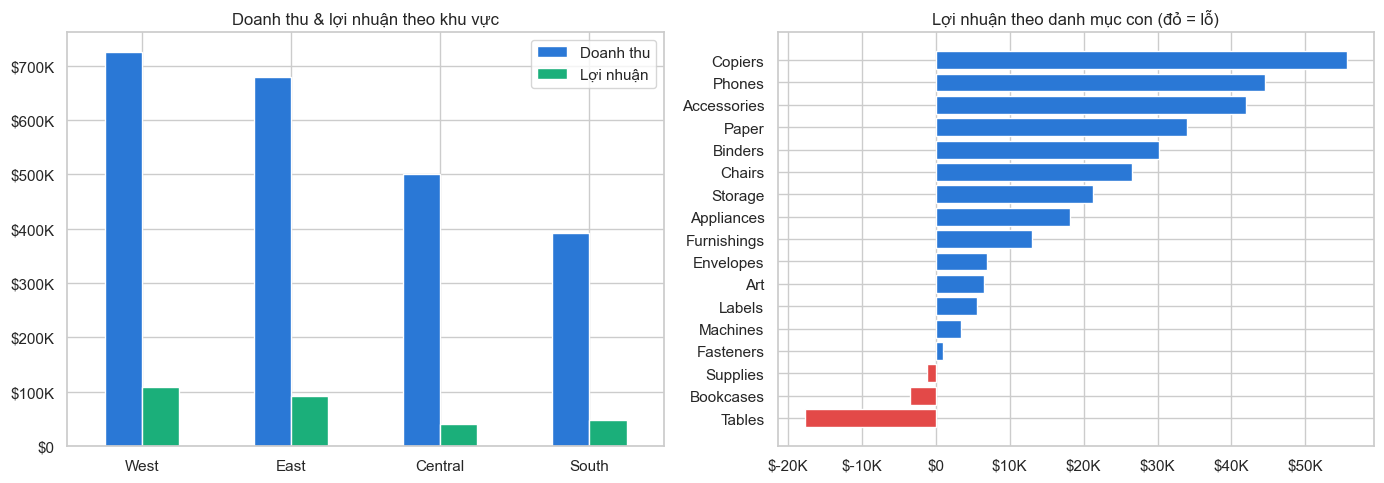
\includegraphics[width=\linewidth]{nb_31_0.png}
\caption{Doanh thu và lợi nhuận theo khu vực (trái); lợi nhuận theo danh mục con (phải, màu đỏ là lỗ)}
\label{fig:sosanh}
\end{figure}
\begin{nhanxet}
West dẫn đầu cả doanh thu (725,5 nghìn USD, 31,6\%) lẫn lợi nhuận (108,4 nghìn USD). Central có doanh thu
đứng thứ ba nhưng biên lợi nhuận thấp nhất (7,9\%). Ba danh mục con \textbf{Tables, Bookcases, Supplies} đang thua lỗ,
riêng Tables lỗ 17,7 nghìn USD dù doanh thu hơn 200 nghìn USD. Copiers và Phones là hai nguồn lợi nhuận lớn nhất.
\end{nhanxet}

\subsection{Biểu đồ phân phối (histogram và boxplot)}
\begin{figure}[H]
\centering
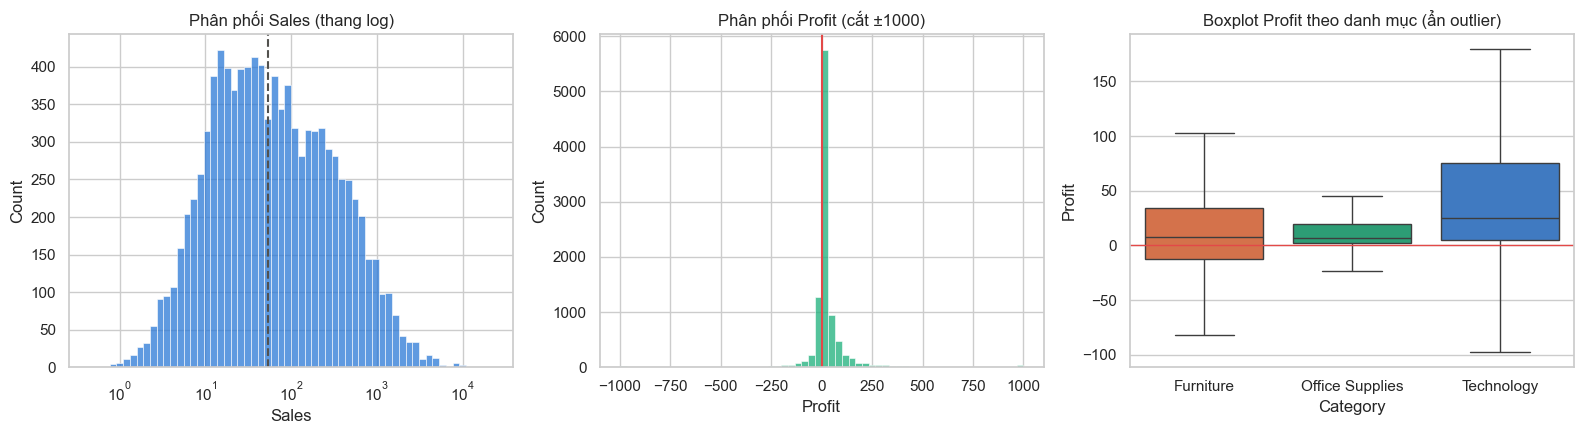
\includegraphics[width=\linewidth]{nb_34_0.png}
\caption{Phân phối Sales (thang log), phân phối Profit và boxplot Profit theo danh mục}
\label{fig:phanphoi}
\end{figure}
\begin{figure}[H]
\centering
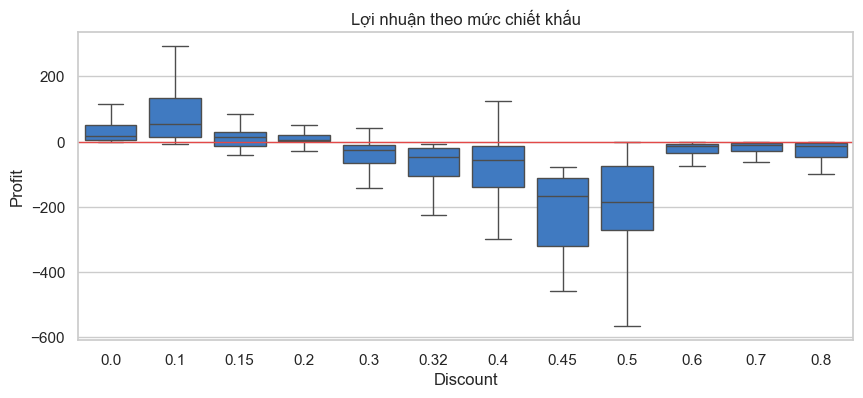
\includegraphics[width=0.85\linewidth]{nb_35_0.png}
\caption{Boxplot lợi nhuận theo mức chiết khấu}
\label{fig:chietkhau}
\end{figure}
\begin{nhanxet}
Trên thang log, doanh thu mỗi dòng có dạng gần chuông, trung vị khoảng 54 USD. Lợi nhuận tập trung quanh 0–30 USD
nhưng có đuôi âm dài. Furniture là danh mục duy nhất có tứ phân vị dưới (Q1) âm (−12,85 USD), tức hơn một phần tư số dòng Furniture bị lỗ. Từ mức chiết khấu
\textbf{30\% trở lên, lợi nhuận trung bình chuyển sang âm}; tệ nhất ở mức 45–50\% (khoảng −227 đến −311 USD/dòng).
\end{nhanxet}

\subsection{Biểu đồ xu hướng theo thời gian}
\begin{figure}[H]
\centering
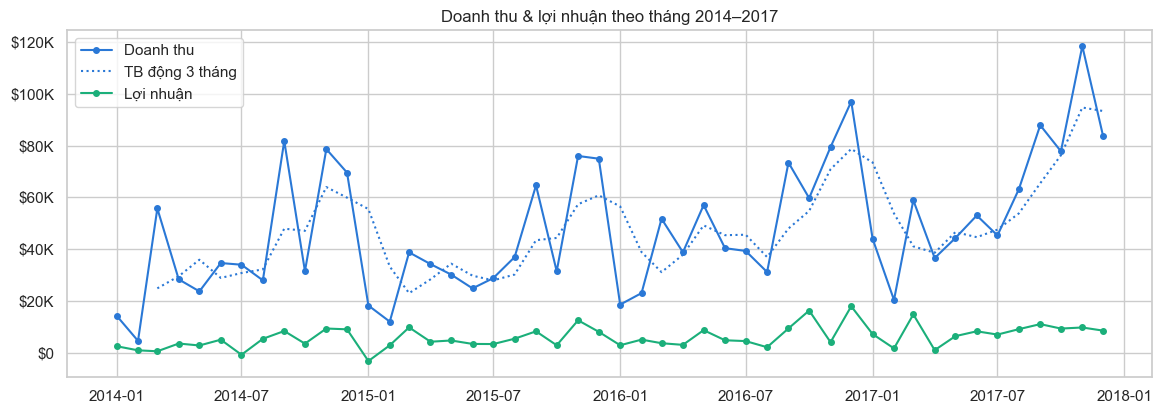
\includegraphics[width=\linewidth]{nb_38_0.png}
\caption{Doanh thu và lợi nhuận theo tháng 2014–2017, kèm trung bình động 3 tháng}
\label{fig:xuhuong}
\end{figure}
\begin{figure}[H]
\centering
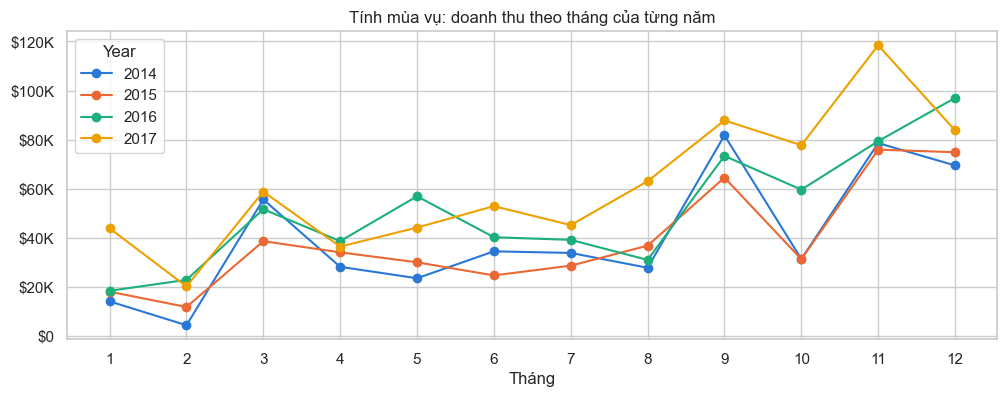
\includegraphics[width=0.9\linewidth]{nb_39_0.png}
\caption{Tính mùa vụ: doanh thu theo tháng của từng năm}
\label{fig:muavu}
\end{figure}
\begin{nhanxet}
Doanh thu có xu hướng \textbf{tăng}: năm 2017 cao hơn năm 2014 khoảng 51\% (tăng trưởng kép 14,8\%/năm),
riêng năm 2015 giảm nhẹ 2,8\%. Tính mùa vụ rất rõ: đỉnh vào \textbf{tháng 9, 11 và 12}, đáy vào tháng 1–2.
Tháng cao nhất là 11/2017 (118,4 nghìn USD), thấp nhất là 02/2014 (4,5 nghìn USD). Quý 4 chiếm \textbf{38,2\%} doanh thu cả giai đoạn.
\end{nhanxet}

\subsection{Biểu đồ tổng hợp (grouped và stacked)}
\begin{figure}[H]
\centering
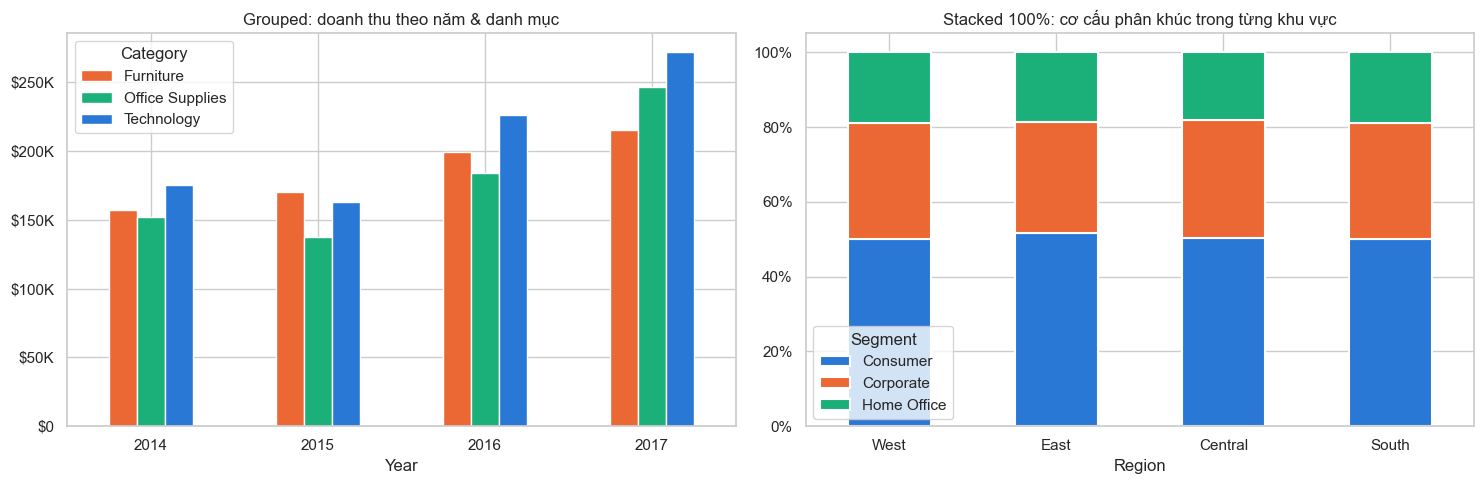
\includegraphics[width=\linewidth]{nb_42_0.png}
\caption{Grouped bar: doanh thu theo năm và danh mục (trái); stacked 100\%: cơ cấu phân khúc theo khu vực (phải)}
\label{fig:tonghop}
\end{figure}
\begin{nhanxet}
Từ 2015 đến 2017, doanh thu cả ba danh mục đều tăng (năm 2015 Office Supplies và Technology giảm nhẹ so với 2014). Technology dẫn đầu ở 3/4 năm, riêng năm 2015 Furniture dẫn đầu. Cơ cấu phân khúc khá
đồng đều giữa các vùng: \textbf{Consumer luôn chiếm khoảng một nửa} doanh thu. Vì vậy, khác biệt giữa các khu vực
đến từ quy mô và mức lợi nhuận, không đến từ tập khách hàng.
\end{nhanxet}

\subsection{Biểu đồ bổ sung: heatmap biên lợi nhuận}
\begin{figure}[H]
\centering
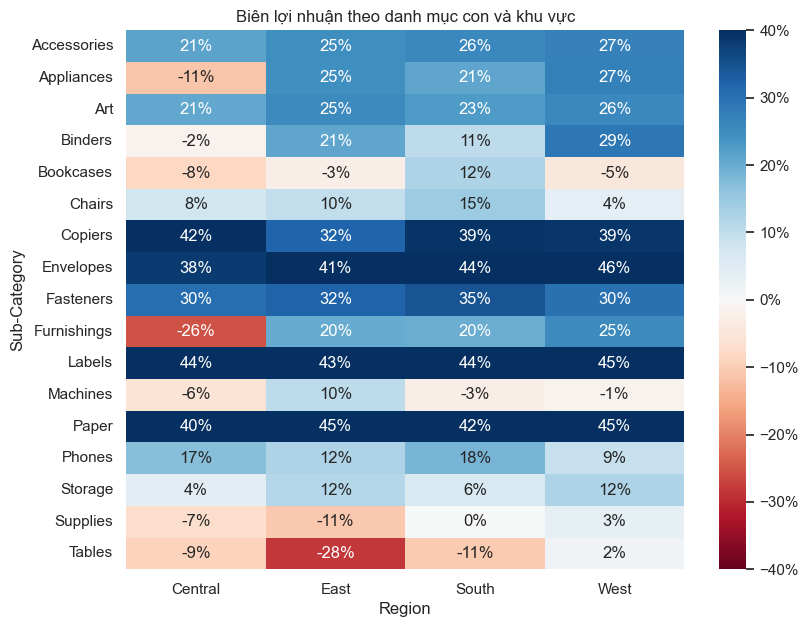
\includegraphics[width=0.75\linewidth]{nb_45_0.png}
\caption{Biên lợi nhuận theo danh mục con và khu vực}
\label{fig:heatmap}
\end{figure}
\begin{nhanxet}
Heatmap chỉ ra chính xác chỗ đang lỗ: \textbf{Tables tại East (−28\%)}, \textbf{Furnishings tại Central (−26\%)},
Appliances tại Central (−11\%), Supplies tại East (−11\%). Paper, Labels, Envelopes và Copiers có biên trên 30\% ở mọi khu vực.
\end{nhanxet}

% ----------------------------- PHẦN 5 -----------------------------
\section{Dashboard tương tác}

\subsection{Kiến trúc hệ thống}
Dashboard là một ứng dụng Streamlit nhiều trang. Mã nguồn được tách thành phần \textit{xử lý dữ liệu}
(\texttt{utils.py}) và phần \textit{giao diện} (thư mục \texttt{pages/}):
\begin{Verbatim}
BTL/
|-- app.py              # Trang chủ, điểm khởi động ứng dụng
|-- utils.py            # Đọc dữ liệu (cache), bộ lọc dùng chung, định dạng
|-- pages/
|   |-- 1_Tong_quan.py   # Page 1 - Tổng quan kinh doanh
|   |-- 2_Xu_huong.py    # Page 2 - Xu hướng theo thời gian
|   |-- 3_Khu_vuc.py     # Page 3 - Phân tích khu vực
|   |-- 4_San_pham.py    # Page 4 - Phân tích sản phẩm
|   |-- 5_Trai_nghiem.py # Page 5 - Khám phá & trải nghiệm
|-- data/superstore.csv  # Dữ liệu gốc
|-- eda.ipynb           # Notebook EDA
|-- requirements.txt    # Thư viện cần cài
\end{Verbatim}

Luồng dữ liệu khi người dùng thao tác:
\begin{center}
\fcolorbox{black!50}{nennhat}{\parbox{0.92\linewidth}{\centering\small
\texttt{superstore.csv} $\rightarrow$ \texttt{load\_data()} (đọc + cache) $\rightarrow$
\texttt{get\_filtered()} (bộ lọc sidebar) $\rightarrow$ \texttt{pages/*.py} (groupby, pivot, Plotly) $\rightarrow$ trình duyệt}}
\end{center}

Các kỹ thuật chính:
\begin{itemize}
  \item \textbf{Bộ lọc dùng chung:} hàm \texttt{get\_filtered()} tạo bộ lọc ở sidebar gồm khoảng thời gian, khu vực,
        danh mục và phân khúc. Trang 5 có thêm bộ lọc nâng cao theo hình thức giao và danh mục con. Mọi trang gọi
        cùng một hàm nên kết quả luôn nhất quán.
  \item \textbf{Giữ trạng thái khi chuyển trang:} giá trị bộ lọc được lưu trong \texttt{st.session\_state}. Có nút
        “Đặt lại bộ lọc”, và dashboard nhắc người dùng khi một bộ lọc bị bỏ trống.
  \item \textbf{Hiệu năng:} \texttt{@st.cache\_data} giúp chỉ đọc file CSV một lần cho mọi lượt tương tác.
  \item \textbf{Nhận xét động:} dưới mỗi biểu đồ có 1–2 câu nhận xét được \textbf{tính lại theo bộ lọc hiện tại},
        không ghi cứng con số.
  \item \textbf{Giao diện nhất quán:} mỗi thực thể (khu vực, danh mục, phân khúc) giữ cố định một màu trên mọi trang;
        lãi màu xanh, lỗ màu đỏ; hỗ trợ cả giao diện sáng và tối.
\end{itemize}

\begin{figure}[H]
\centering
\anh[0.85\linewidth]{p0_home.jpg}
\caption{Trang chủ dashboard với menu điều hướng 5 trang}
\label{fig:home}
\end{figure}

\subsection{Page 1 – Tổng quan kinh doanh}
\textbf{Mục tiêu:} cho khách hàng nhìn nhanh toàn cảnh kinh doanh.\\
\textbf{Thành phần:} 8 chỉ số KPI bằng \texttt{st.metric} (tổng doanh thu, số đơn hàng, số sản phẩm đã bán,
tổng lợi nhuận, biên lợi nhuận, số khách hàng, giá trị trung bình mỗi đơn, số lượng bán), kèm mức thay đổi
so với kỳ trước có cùng độ dài. Bên dưới là bảng groupby và biểu đồ cột theo danh mục và phân khúc,
cùng ma trận Danh mục × Phân khúc.
\begin{figure}[H]
\centering
\anh[0.62\linewidth]{p1_a.jpg}\\[6pt]
\anh[0.62\linewidth]{p1_b.jpg}
\caption{Page 1 – KPI tổng quan (trên), groupby theo danh mục và phân khúc (dưới)}
\label{fig:p1}
\end{figure}
\textbf{Insight:} doanh thu 2,30 triệu USD, lợi nhuận 286,4 nghìn USD (biên 12,5\%) từ 5.009 đơn của 793 khách hàng,
giá trị trung bình 459 USD/đơn. Technology dẫn đầu doanh thu (36,4\%) và biên lợi nhuận (17,4\%), còn Furniture
chỉ đạt biên 2,5\%.

\subsection{Page 2 – Xu hướng doanh thu theo thời gian}
\textbf{Mục tiêu:} trả lời câu hỏi doanh thu tăng hay giảm.\\
\textbf{Thành phần:} line chart Plotly cho doanh thu và lợi nhuận. Người dùng chọn độ chi tiết theo tháng, quý hoặc năm,
và có thể bật đường trung bình động. Khoảng thời gian được lọc bằng \texttt{date\_input} ở sidebar.
Trang còn có biểu đồ tăng trưởng theo năm, biểu đồ so sánh mùa vụ giữa các năm và xu hướng theo từng nhóm
(danh mục, khu vực, phân khúc).
\begin{figure}[H]
\centering
\anh[0.62\linewidth]{p2_a.jpg}\\[6pt]
\anh[0.62\linewidth]{p2_b.jpg}
\caption{Page 2 – Xu hướng theo tháng (trên), tăng trưởng năm và tính mùa vụ (dưới)}
\label{fig:p2}
\end{figure}
\textbf{Insight:} doanh thu tăng trưởng kép 14,8\%/năm. Năm 2016 tăng mạnh nhất (+29,5\%), năm 2015 giảm nhẹ (−2,8\%).
Các tháng 9, 11, 12 là mùa cao điểm; quý 4 chiếm 38,2\% doanh thu.

\subsection{Page 3 – Phân tích theo khu vực}
\textbf{Mục tiêu:} xác định khu vực hoạt động tốt nhất.\\
\textbf{Thành phần:} ô \texttt{multiselect} chọn khu vực ở đầu trang; thẻ KPI cho từng khu vực; bar chart doanh thu,
lợi nhuận và biên lợi nhuận theo khu vực (dữ liệu tổng hợp bằng groupby); Top N bang có thanh trượt chọn N;
bản đồ doanh thu theo bang; danh sách các bang thua lỗ kèm mức chiết khấu trung bình.
\begin{figure}[H]
\centering
\anh[0.62\linewidth]{p3_a.jpg}\\[6pt]
\anh[0.62\linewidth]{p3_b.jpg}
\caption{Page 3 – So sánh khu vực (trên), chi tiết theo bang và bản đồ (dưới)}
\label{fig:p3}
\end{figure}
\textbf{Insight:} \textbf{West là khu vực nổi bật nhất}: doanh thu cao nhất (31,6\%) và biên lợi nhuận cao nhất (14,9\%).
Central bán được hàng nhưng biên chỉ 7,9\%, đi cùng mức chiết khấu trung bình cao nhất (24\%).
California và New York chiếm 33,5\% doanh thu. Có 10 bang thua lỗ (tổng −98,2 nghìn USD), nặng nhất là Texas (−25,7 nghìn USD).

\subsection{Page 4 – Phân tích sản phẩm}
\textbf{Mục tiêu:} tìm sản phẩm mang lại doanh thu cao.\\
\textbf{Thành phần:} Top N sản phẩm (thanh trượt chọn N), biểu đồ cột ngang, xem theo sản phẩm hoặc danh mục con,
xếp hạng theo doanh thu, lợi nhuận hoặc số lượng; lọc theo thời gian và khu vực qua sidebar.
Trang có thêm biểu đồ lợi nhuận theo danh mục con, tác động của mức chiết khấu, và \textbf{pivot table dạng heatmap}
Danh mục (hoặc danh mục con) × Khu vực.
\begin{figure}[H]
\centering
\anh[0.62\linewidth]{p4_a.jpg}\\[6pt]
\anh[0.62\linewidth]{p4_b.jpg}
\caption{Page 4 – Top 10 sản phẩm (trên), lợi nhuận danh mục con và heatmap pivot (dưới)}
\label{fig:p4}
\end{figure}
\textbf{Insight:} Top 10 sản phẩm chiếm 10,6\% doanh thu, dẫn đầu là máy photocopy Canon imageCLASS 2200 (61,6 nghìn USD).
Office Supplies xuất hiện nhiều nhất trong Top 10 (5/10). Có 3 sản phẩm trong Top 10 bị lỗ, cho thấy doanh thu
cao chưa chắc mang lại lợi nhuận.

\subsection{Page 5 – Khám phá và trải nghiệm người dùng}
\textbf{Mục tiêu:} giúp người không chuyên dùng được dashboard.\\
\textbf{Thành phần:} sidebar chứa toàn bộ bộ lọc (kể cả bộ lọc nâng cao). Nội dung chia thành 4 tab:
(1) \textit{Hướng dẫn sử dụng}, gồm 3 bước dùng dashboard và các expander giải thích chỉ số, câu hỏi thường gặp;
(2) \textit{Phân phối dữ liệu}, gồm histogram và boxplot có tùy chọn trục log;
(3) \textit{So sánh nhóm}, gồm biểu đồ grouped, stacked và stacked 100\%;
(4) \textit{Tra cứu dữ liệu}, gồm bảng dữ liệu đã lọc và nút tải CSV.
\begin{figure}[H]
\centering
\anh[0.62\linewidth]{p5_a.jpg}\\[6pt]
\anh[0.62\linewidth]{p5_b.jpg}
\caption{Page 5 – Tab hướng dẫn sử dụng (trên), tab phân phối dữ liệu (dưới)}
\label{fig:p5}
\end{figure}
\begin{figure}[H]
\centering
\anh[0.62\linewidth]{p5_c.jpg}
\caption{Page 5 – Tab so sánh nhóm (grouped bar)}
\label{fig:p5c}
\end{figure}

\subsection{Đối chiếu với yêu cầu đề bài}
\begin{table}[H]
\centering
\caption{Đối chiếu yêu cầu bắt buộc với dashboard}\label{tab:doichieu}
\small
\begin{tabularx}{\linewidth}{@{}l Y c@{}}
\toprule
\textbf{Page} & \textbf{Yêu cầu bắt buộc} & \textbf{Đáp ứng} \\
\midrule
1 & KPI tổng doanh thu, số đơn, số sản phẩm bằng \texttt{st.metric}; groupby; trình bày gọn & \checkmark \\
2 & Line chart Plotly; lọc thời gian bằng \texttt{date\_input}; cập nhật theo tương tác & \checkmark \\
3 & Bar chart so sánh khu vực; groupby; \texttt{multiselect} nhiều khu vực; nhận xét khu vực nổi bật & \checkmark \\
4 & Top N sản phẩm; biểu đồ cột ngang; lọc thời gian/khu vực; pivot table & \checkmark \\
5 & Sidebar chứa toàn bộ bộ lọc; tabs/expander; giao diện dễ hiểu; cache & \checkmark \\
Chung & Sidebar filter ≥ 2 điều kiện; tabs/columns; biểu đồ cập nhật theo tương tác & \checkmark \\
\bottomrule
\end{tabularx}
\end{table}

% ----------------------------- PHẦN 6 -----------------------------
\section{Nhận xét, insight và đề xuất}

\subsection{Các phát hiện chính}
\begin{enumerate}
  \item \textbf{Quy mô và hiệu quả:} doanh thu 2,30 triệu USD, lợi nhuận 286,4 nghìn USD, biên lợi nhuận 12,5\%.
        Cứ 100 USD bán ra, doanh nghiệp giữ lại khoảng 12,5 USD.
  \item \textbf{Tăng trưởng và mùa vụ:} doanh thu tăng 51\% từ 2014 đến 2017 (14,8\%/năm). Quý 4 chiếm 38,2\%
        doanh thu, đỉnh vào tháng 9, 11, 12.
  \item \textbf{Khu vực:} West và East chiếm khoảng 61\% doanh thu. Central có biên thấp nhất (7,9\%) và chiết khấu
        trung bình cao nhất (24\%).
  \item \textbf{Bang thua lỗ:} 10 bang lỗ tổng cộng 98,2 nghìn USD. Lỗ nặng nhất là Texas (−25,7 nghìn), Ohio (−17,0 nghìn),
        Pennsylvania (−15,6 nghìn) và Illinois (−12,6 nghìn).
  \item \textbf{Sản phẩm:} Furniture có doanh thu cao (32,3\%) nhưng biên chỉ 2,5\%. Tables, Bookcases và Supplies thua lỗ;
        Machines gần như hòa vốn (biên 1,8\%). Copiers, Paper, Labels, Envelopes có biên trên 37\%.
  \item \textbf{Chiết khấu:} từ mức chiết khấu 30\% trở lên, lợi nhuận trung bình mỗi dòng chuyển sang âm.
        922 dòng có chiết khấu từ 50\% trở lên lỗ trung bình 105 USD/dòng.
  \item \textbf{Khách hàng:} Consumer đóng góp 50,6\% doanh thu, nhưng Home Office có biên lợi nhuận cao nhất (14,0\%).
\end{enumerate}

\subsection{Gợi ý ra quyết định}
\begin{table}[H]
\centering
\caption{Phát hiện và gợi ý quyết định cho doanh nghiệp}\label{tab:dexuat}
\small
\begin{tabularx}{\linewidth}{@{}c Y Y@{}}
\toprule
\textbf{\#} & \textbf{Phát hiện} & \textbf{Gợi ý quyết định} \\
\midrule
1 & Chiết khấu ≥ 30\% làm lợi nhuận trung bình âm
  & Đặt trần chiết khấu khoảng 20\%; chiết khấu cao hơn cần quản lý phê duyệt. \\
2 & Central và các bang Texas, Ohio, Pennsylvania, Illinois lỗ nặng
  & Rà soát chính sách giá và chiết khấu tại các bang này, ưu tiên Texas. \\
3 & Tables, Bookcases lỗ; Furniture biên chỉ 2,5\%
  & Tăng giá hoặc giảm khuyến mãi cho bàn và kệ sách; xem lại chi phí vận chuyển hàng cồng kềnh. \\
4 & Copiers, Phones, Accessories, Paper sinh lời cao
  & Ưu tiên quảng bá, bán kèm (cross-sell) các nhóm này. \\
5 & Quý 4 chiếm 38\% doanh thu
  & Chuẩn bị tồn kho, nhân sự và chiến dịch marketing từ tháng 9; dùng tháng 1–2 cho khuyến mãi kích cầu có kiểm soát. \\
6 & Home Office có biên cao nhất nhưng tỷ trọng nhỏ (18,7\%)
  & Phát triển phân khúc Home Office bằng gói sản phẩm văn phòng tại nhà. \\
7 & Doanh thu cao chưa chắc có lãi (3 sản phẩm Top 10 bị lỗ)
  & Theo dõi biên lợi nhuận song song với doanh thu trong mọi báo cáo. \\
\bottomrule
\end{tabularx}
\end{table}


% ============================ KẾT LUẬN ===============================
\TieuDeLon{KẾT LUẬN}
Bài tập lớn đã xây dựng hoàn chỉnh quy trình từ dữ liệu thô đến dashboard hỗ trợ ra quyết định cho doanh nghiệp
bán lẻ Superstore. Dưới đây là đánh giá ưu điểm, nhược điểm và hướng phát triển của sản phẩm.

\subsection*{1. Ưu điểm}
\begin{itemize}
  \item Mô tả dữ liệu và EDA đầy đủ: dữ liệu thiếu và trùng lặp, ngoại lệ theo IQR, thống kê mô tả,
        lọc theo điều kiện, groupby, pivot table.
  \item Có đủ bốn loại biểu đồ bắt buộc, mỗi biểu đồ đi kèm nhận xét rút ra từ số liệu thật.
  \item Dashboard Streamlit 5 trang liên kết với nhau qua bộ lọc dùng chung. Biểu đồ cập nhật theo tương tác,
        có nhận xét động, hỗ trợ giao diện sáng và tối, dữ liệu được cache nên phản hồi nhanh.
  \item Rút ra 7 phát hiện chính và gợi ý quyết định cụ thể cho doanh nghiệp.
\end{itemize}

\subsection*{2. Nhược điểm}
\begin{itemize}
  \item Dữ liệu chỉ gồm 4 năm và một quốc gia, không có thông tin chi phí chi tiết (vận chuyển, giá vốn),
        nên chưa giải thích được đầy đủ nguyên nhân thua lỗ.
  \item Dashboard đang chạy cục bộ, chưa triển khai lên máy chủ để nhiều người cùng truy cập.
\end{itemize}

\subsection*{3. Hướng phát triển}
\begin{itemize}
  \item Triển khai dashboard lên Streamlit Community Cloud để chia sẻ qua đường link.
  \item Bổ sung dự báo doanh thu theo mùa vụ (mô hình chuỗi thời gian) và phân tích RFM cho khách hàng.
  \item Mô phỏng tác động của việc giới hạn mức chiết khấu lên lợi nhuận.
\end{itemize}

% ============================ TÀI LIỆU THAM KHẢO ===============================
\clearpage
\phantomsection\addcontentsline{toc}{section}{DANH MỤC TÀI LIỆU THAM KHẢO}

\begin{thebibliography}{9}
\bibitem{kaggle} vivek468 (Kaggle user), \textit{Superstore Dataset}, Kaggle.
  \url{https://www.kaggle.com/datasets/vivek468/superstore-dataset-final}
\end{thebibliography}

% ============================ PHỤ LỤC ===============================
\TieuDeLon{PHỤ LỤC}
\subsection*{A. Mã nguồn}
Mã nguồn trên GitHub: \texttt{[đường dẫn repository]}.

\subsection*{B. Phân công công việc}
\begin{table}[H]
\centering
\caption*{Phân công công việc trong nhóm}
\renewcommand{\arraystretch}{1.3}
\begin{tabularx}{\linewidth}{|c|l|Y|c|}
\hline
\textbf{STT} & \textbf{Họ và tên} & \textbf{Công việc} & \textbf{Mức đóng góp} \\ \hline
1 & Ngô Ngọc Sang & Phân tích đề bài, thu thập dữ liệu; xây dựng bộ lọc dùng chung (utils.py) và Page 1 – Tổng quan; tổng hợp, trình bày báo cáo LaTeX & 25\% \\ \hline
2 & Lê Thanh Đại & Khám phá dữ liệu (EDA): dữ liệu thiếu, ngoại lệ, thống kê mô tả, groupby, pivot; Page 2 – Xu hướng; viết mục 2–3 báo cáo & 25\% \\ \hline
3 & Đỗ Quang Chính & Trực quan hóa 4 loại biểu đồ bắt buộc; Page 3 – Khu vực; viết mục 4 báo cáo; làm slide thuyết trình & 25\% \\ \hline
4 & Võ Ngọc Hải & Page 4 – Sản phẩm và Page 5 – Trải nghiệm người dùng; rút ra insight, đề xuất; viết mục 5–6 báo cáo, kịch bản demo & 25\% \\ \hline
\end{tabularx}
\end{table}

\end{document}
